\documentclass{standalone}

\usepackage{times}
\usepackage{amsmath}
\usepackage{amssymb}

\usepackage[dvipsnames]{xcolor}
\usepackage{tikz}
\usetikzlibrary{arrows,calc}
\pgfdeclarelayer{background}
\pgfdeclarelayer{foreground}
\pgfsetlayers{background,main,foreground}

\usepackage{pgfplots}
\pgfplotsset{compat=1.15}

\definecolor{red}{HTML}{cf555a}
\newcounter{nextCircle}
\setcounter{nextCircle}{1}

\begin{document}
	\Large
	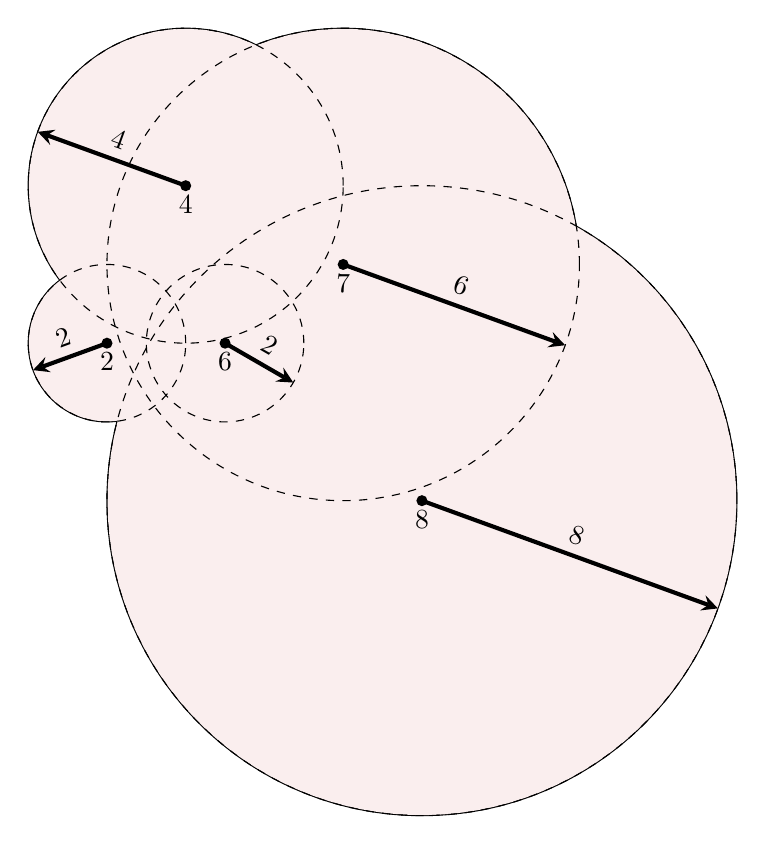
\begin{tikzpicture}[x=0.5cm,y=0.5cm]
		\newcommand{\addCircle}[5][]{
			\begin{pgfonlayer}{background}
				\fill[black,#1] (#2) circle (#4*0.5cm+0.2pt);
			\end{pgfonlayer}
			\fill[red!10,#1] (#2) circle (#4*0.5cm-0.2pt);
			\begin{pgfonlayer}{foreground}
				\draw[dashed,#1] (#2) circle (#4);
				\fill[black] (#2) circle (2pt);
				\node[anchor=north] at (#2) {#3};
				\draw[line width=1.5pt,-stealth] (#2) -- ($(#2)+(#5:#4)$) node [midway, above, sloped] {#4};
			\end{pgfonlayer}
			\stepcounter{nextCircle}
		}
		
		\addCircle{2,6}{2}{2}{200}
		\addCircle{4,10}{4}{4}{160}
		\addCircle{5,6}{6}{2}{330}
		\addCircle{8,8}{7}{6}{-20}
		\addCircle{10,2}{8}{8}{-20}
	\end{tikzpicture}
\end{document} 
